% Generated from reviewed lane; compile via book/textbook.tex.
\clearpage

原书 PDF 页 119；印刷页码 106。

\href{source-images/pdf-119.jpeg}{原页}

\section{第 5 章 常微分方程数值解法}\label{ch05a-ux7b2c-5-ux7ae0-ux5e38ux5faeux5206ux65b9ux7a0bux6570ux503cux89e3ux6cd5}

\subsection{5.1 引言}\label{ch05a-ux5f15ux8a00}

科学技术中常常需要求解常微分方程的定解问题。这类问题最简单的形式，是本章将要着重考察的一阶方程的初值问题

\[
y'=f(x,y),\tag{5.1.1}
\]

\[
y(x_0)=y_0.\tag{5.1.2}
\]

我们知道，只要函数 \(f(x,y)\) 适当光滑------譬如关于 \(y\) 满足 Lipschitz 条件

\[
|f(x,y)-f(x,\bar y)|\leqslant L|y-\bar y|,
\]

理论上就可以保证初值问题 (5.1.1)、(5.1.2) 的解 \(y=y(x)\) 存在并且唯一。

虽然求解常微分方程有各种各样的解析方法，但解析方法只能用来求解一些特殊类型的方程，实际问题中归结出来的微分方程主要靠数值解法求解。

所谓\textbf{数值解法}，就是寻求解 \(y(x)\) 在一系列离散节点

\[
x_1<x_2<\cdots<x_n<x_{n+1}<\cdots
\]

上的近似值 \(y_1,\allowbreak y_2,\allowbreak \cdots,\allowbreak y_n,\allowbreak y_{n+1},\allowbreak \cdots\)。相邻两个节点的间距 \(h=x_{n+1}-x_n\) 称为\textbf{步长}。今后如不特别说明，总是假定 \(h\) 为定数，这时节点为 \(x_n=x_0+nh\)，\(n=0,1,2,\cdots\)。

初值问题 (5.1.1)、(5.1.2) 的数值解法有个基本特点，它们都采取``步进式''，即求解过程顺着节点排列的次序一步一步地向前推进。描述这类算法，只要给出用已知信息 \(y_n,y_{n-1},y_{n-2},\cdots\) 计算 \(y_{n+1}\) 的递推公式即可。这种计算公式称为\textbf{差分格式}。

\subsection{5.2 Euler 方法}\label{ch05a-euler-ux65b9ux6cd5}

\subsubsection{5.2.1 Euler 格式}\label{ch05a-euler-ux683cux5f0f}

我们知道，在 \(Oxy\) 平面上，微分方程 (5.1.1) 的解 \(y=y(x)\) 称为它的\textbf{积分曲线}。积分曲线上一点 \((x,y)\) 的切线斜率等于函数 \(f(x,y)\) 的值。如果按函数 \(f(x,y)\) 在 \(Oxy\) 平面上建立一个方向场，那么，积分曲线上每一点的切线方向均与方向场在该点的方向一致。

基于上述几何解释，我们从初始点 \(P_0(x_0,y_0)\) 出发，先依方向场在该点的方向推

\clearpage

原书 PDF 页 120；印刷页码 107。

\href{source-images/pdf-120.jpeg}{原页}

进到 \(x=x_1\) 上一点 \(P_1\)，然后再从 \(P_1\) 依方向场的方向推进到 \(x=x_2\) 上一点 \(P_2\)，循此前进作出一条折线 \(P_0P_1P_2\cdots\)（见图 5.1）。

一般地，设已作出该折线的极点 \(P_n\)，过 \(P_n(x_n,y_n)\) 依方向场的方向再推进到 \(P_{n+1}(x_{n+1},y_{n+1})\)，显然两个极点 \(P_n,P_{n+1}\) 的坐标有下列关系：

\[
\frac{y_{n+1}-y_n}{x_{n+1}-x_n}=f(x_n,y_n),
\]

即

\[
y_{n+1}=y_n+hf(x_n,y_n).\tag{5.2.1}
\]

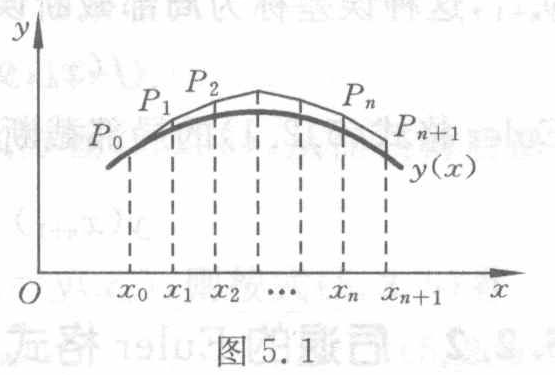
\includegraphics[width=0.85\linewidth,height=\textheight,keepaspectratio,alt={图 5.1 原图}]{verified/assets/ch05a/fig-5.1.png}

图 5.1（原图）：Euler 折线 \(P_0P_1P_2\cdots P_nP_{n+1}\) 与积分曲线 \(y(x)\)。原图符号标签：\(O,\allowbreak x,\allowbreak y,\allowbreak x_0,\allowbreak x_1,\allowbreak x_2,\allowbreak \cdots,\allowbreak x_n,\allowbreak x_{n+1},\allowbreak P_0,\allowbreak P_1,\allowbreak P_2,\allowbreak P_n,\allowbreak P_{n+1},\allowbreak y(x)\)。

这就是著名的 \textbf{Euler 格式}。若初值 \(y_0\) 已知，则依格式 (5.2.1) 可逐步算出

\[
y_1=y_0+hf(x_0,y_0),\qquad y_2=y_1+hf(x_1,y_1),\qquad\cdots.
\]

\textbf{例 5.1} 求解初值问题

\[
\begin{cases}
y'=y-2x/y\quad(0<x<1),\\
y(0)=1.
\end{cases}\tag{5.2.2}
\]

\textbf{解} 为便于比较，本章将用多种数值方法求解上述初值问题。这里先用 Euler 方法，Euler 格式的具体形式为

\[
y_{n+1}=y_n+h\left(y_n-\frac{2x_n}{y_n}\right).
\]

取步长 \(h=0.1\)，计算结果如表 5.1 所示。

\textbf{表 5.1}

{\def\LTcaptype{none} % do not increment counter
\begin{longtable}[]{@{}llllll@{}}
\toprule\noalign{}
\(x_n\) & \(y_n\) & \(y(x_n)\) & \(x_n\) & \(y_n\) & \(y(x_n)\) \\
\midrule\noalign{}
\endhead
\bottomrule\noalign{}
\endlastfoot
0.1 & 1.1000 & 1.0954 & 0.6 & 1.5090 & 1.4832 \\
0.2 & 1.1918 & 1.1832 & 0.7 & 1.5803 & 1.5492 \\
0.3 & 1.2774 & 1.2649 & 0.8 & 1.6498 & 1.6125 \\
0.4 & 1.3582 & 1.3416 & 0.9 & 1.7178 & 1.6733 \\
0.5 & 1.4351 & 1.4142 & 1.0 & 1.7848 & 1.7321 \\
\end{longtable}
}

初值问题 (5.2.2) 有解 \(y=\sqrt{1+2x}\)，按这个解析式子算出的准确值 \(y(x_n)\) 同近似值 \(y_n\) 一起列在表 5.1 中，二者相比较可以看出，Euler 方法的精度很差。

还可以通过几何直观来考察 Euler 方法的精度。假设 \(y_n=y(x_n)\)，即顶点 \(P_n\) 落在积分曲线 \(y=y(x)\) 上，那么，按 Euler 方法作出的折线 \(P_nP_{n+1}\) 便是 \(y=y(x)\) 过点 \(P_n\) 的切线（见图 5.2）。从图形上看，这样定出的顶点 \(P_{n+1}\) 显著地偏离了原来的积分曲线，可见 Euler 方法是相当粗糙的。

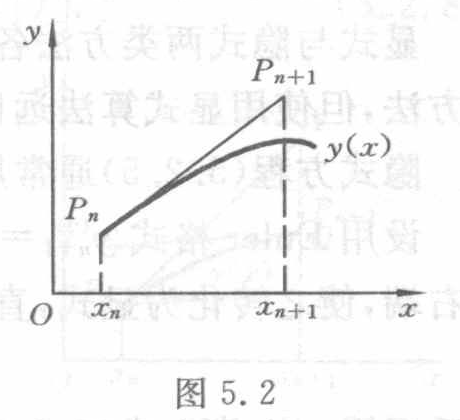
\includegraphics[width=0.85\linewidth,height=\textheight,keepaspectratio,alt={图 5.2 原图}]{verified/assets/ch05a/fig-5.2.png}

图 5.2（原图）：从积分曲线上 \(P_n\) 沿切线得到 \(P_{n+1}\)，与曲线 \(y(x)\) 在 \(x_{n+1}\) 的值有偏差。原图符号标签：\(O,\allowbreak x,\allowbreak y,\allowbreak x_n,\allowbreak x_{n+1},\allowbreak P_n,\allowbreak P_{n+1},\allowbreak y(x)\)。

人们常以 Taylor 展开为工具来分析计算公式的

\clearpage

原书 PDF 页 121；印刷页码 108。

\href{source-images/pdf-121.jpeg}{原页}

精度。为简化分析，假定 \(y_n\) 是准确的，即在 \(y_n=y(x_n)\) 的前提下估计误差 \(y(x_{n+1})-y_{n+1}\)，这种误差称为\textbf{局部截断误差}。注意到

\[
f(x_n,y_n)=f(x_n,y(x_n))=y'(x_n),
\]

Euler 格式 (5.2.1) 的局部截断误差显然为

\[
y(x_{n+1})-y_{n+1}=\frac{h^2}{2}y''(\xi)\approx\frac{h^2}{2}y''(x_n).\tag{5.2.3}
\]

\subsubsection{5.2.2 后退的 Euler 格式}\label{ch05a-ux540eux9000ux7684-euler-ux683cux5f0f}

方程 \(y'=f(x,y)\) 中含有导数项 \(y'(x)\)，这是微分方程的本质特征，也正是它难以求解的症结所在。数值解法的关键在于设法消除其导数项，这项手续称为\textbf{离散化}。由于差分是微分的近似运算，实现离散化的基本途径之一是直接用差商替代导数。譬如，若在点 \(x_n\) 列出方程

\[
y'(x_n)=f(x_n,y(x_n)),\tag{5.2.4}
\]

并用差商 \(\dfrac{y(x_{n+1})-y(x_n)}{h}\) 近似替代其中的导数 \(y'(x_n)\)，结果有

\[
y(x_{n+1})\approx y(x_n)+hf(x_n,y(x_n)).
\]

设 \(y(x_n)\) 的近似值 \(y_n\) 已知，用它代入上式右端进行计算，并取计算结果 \(y_{n+1}\) 作为 \(y(x_{n+1})\) 的近似值，这就是 Euler 格式。

对于在点 \(x_{n+1}\) 列出的方程 (5.1.1)，有

\[
y'(x_{n+1})=f(x_{n+1},y(x_{n+1})),
\]

若用向后差商 \(\dfrac{y(x_{n+1})-y(x_n)}{h}\) 替代导数 \(y'(x_{n+1})\)，则可将上式离散化得

\[
\frac{y_{n+1}-y_n}{h}=f(x_{n+1},y_{n+1}),
\]

即

\[
y_{n+1}=y_n+hf(x_{n+1},y_{n+1}),\tag{5.2.5}
\]

此为\textbf{后退的 Euler 格式}。

后退的 Euler 格式与 Euler 格式有着本质的区别，后者是关于 \(y_{n+1}\) 的一个直接的计算格式，这类格式是\textbf{显式的}；而格式 (5.2.5) 的右端含有未知的 \(y_{n+1}\)，它实际上是关于 \(y_{n+1}\) 的一个函数方程，这类格式是\textbf{隐式的}。

显式与隐式两类方法各有特点。考虑到数值稳定性等因素，人们有时需要选用隐式方法，但使用显式算法远比隐式方便。

隐式方程 (5.2.5) 通常用迭代法求解，而迭代过程的实质是逐步显式化。

设用 Euler 格式 \(y_{n+1}^{(0)}=y_n+hf(x_n,y_n)\) 给出迭代初值 \(y_{n+1}^{(0)}\)，用它代入式 (5.2.5) 的右端，使之转化为显式，直接计算得

\[
y_{n+1}^{(1)}=y_n+hf(x_{n+1},y_{n+1}^{(0)}),
\]

然后再用 \(y_{n+1}^{(1)}\) 代入式 (5.2.5) 的右端，又有

\clearpage

原书 PDF 页 122；印刷页码 109。

\href{source-images/pdf-122.jpeg}{原页}

\[
y_{n+1}^{(2)}=y_n+hf(x_{n+1},y_{n+1}^{(1)}).
\]

如此反复进行迭代，得

\[
y_{n+1}^{(k+1)}=y_n+hf(x_{n+1},y_{n+1}^{(k)})\qquad(k=0,1,\cdots).
\]

如果迭代过程收敛，则极限值 \(y_{n+1}=\lim\limits_{k\to\infty}y_{n+1}^{(k)}\) 必满足隐式方程 (5.2.5)，从而获得后退的 Euler 方法的解。

再考察后退的 Euler 格式的局部截断误差。假设 \(y_n=y(x_n)\)，则按式 (5.2.5) 有

\[
y_{n+1}=y(x_n)+hf(x_{n+1},y_{n+1}),\tag{5.2.6}
\]

由于

\[
f(x_{n+1},y_{n+1})=f(x_{n+1},y(x_{n+1}))+f_y(x_{n+1},\eta)[y_{n+1}-y(x_{n+1})],
\]

其中 \(\eta\) 介于 \(y_{n+1}\) 与 \(y(x_{n+1})\) 之间。又

\[
f(x_{n+1},y(x_{n+1}))=y'(x_{n+1})=y'(x_n)+hy''(x_n)+\cdots,
\]

代入式 (5.2.6) 有

\[
y_{n+1}=hf_y(x_{n+1},\eta)[y_{n+1}-y(x_{n+1})]+y(x_n)+hy'(x_n)+h^2y''(x_n)+\cdots,
\]

将它与 Taylor 展开式

\[
y(x_{n+1})=y(x_n)+hy'(x_n)+\frac{h^2}{2}y''(x_n)+\cdots
\]

相减，得

\[
y(x_{n+1})-y_{n+1}=hf_y(x_{n+1},\eta)[y(x_{n+1})-y_{n+1}]-\frac{h^2}{2}y''(x_n)+\cdots.
\]

再注意到

\[
\frac{1}{1-hf_y(x_{n+1},\eta)}=1+hf_y(x_{n+1},\eta)+\cdots,
\]

最后整理，得

\[
y(x_{n+1})-y_{n+1}\approx-\frac{h^2}{2}y''(x_n).\tag{5.2.7}
\]

\subsubsection{5.2.3 梯形格式}\label{ch05a-ux68afux5f62ux683cux5f0f}

比较 Euler 格式与后退的 Euler 格式的误差公式 (5.2.3)、(5.2.7)，可以看到，如果将这两种方法进行算术平均，即可消除误差的主要部分 \(\pm\dfrac{h^2}{2}y''_n\) 而获得更高的精度。这种平均化方法通常称为\textbf{梯形方法}，其计算格式为

\[
y_{n+1}=y_n+\frac{h}{2}[f(x_n,y_n)+f(x_{n+1},y_{n+1})].\tag{5.2.8}
\]

梯形方法的这种平均化思想亦可借助于几何直观来说明，仍设顶点 \(P_n(x_n,y_n)\) 落在积分曲线 \(y=y(x)\) 上（见图 5.3），用 Euler 方法求解时，过点 \(P_n\) 以斜率 \(f(x_n,y_n)\) 引折线交 \(x=x_{n+1}\) 得出顶点 \(A\)，而用后退的 Euler 方法求解时，则以点 \(Q(x_{n+1},y_{n+1})\) 的斜率 \(f(x_{n+1},y_{n+1})\) 从顶点 \(P_n\) 引折线交 \(x=x_{n+1}\) 得另一顶点 \(B\)。\(A\) 和 \(B\) 两点均偏离

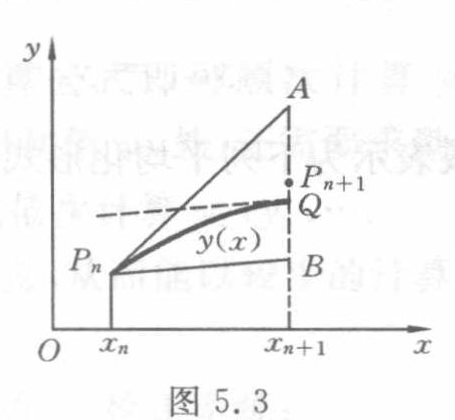
\includegraphics[width=0.85\linewidth,height=\textheight,keepaspectratio,alt={图 5.3 原图}]{verified/assets/ch05a/fig-5.3.png}

图 5.3（原图）：\(P_n\) 出发的两条线分别交 \(x=x_{n+1}\) 于 \(A,B\)，取平均所得点为 \(P_{n+1}\)；积分曲线标为 \(y(x)\)。原图全部标签：\(O,\allowbreak x,\allowbreak y,\allowbreak x_n,\allowbreak x_{n+1},\allowbreak P_n,\allowbreak A,\allowbreak B,\allowbreak P_{n+1},\allowbreak Q,\allowbreak y(x)\)。

\clearpage

原书 PDF 页 123；印刷页码 110。

\href{source-images/pdf-123.jpeg}{原页}

点 \(Q\) 比较远，然而从图形上可以明显地看出，\(AB\) 的中点 \(P_{n+1}\) 相当接近点 \(Q\)，可见梯形方法确实改善了精度（这里的解释不够严密，然而是令人信服的）。

梯形方法是隐式的，可用迭代法求解。同后退的 Euler 方法一样，仍用 Euler 方法提供迭代初值，则梯形法的迭代公式为

\[
\begin{cases}
y_{n+1}^{(0)}=y_n+hf(x_n,y_n),\\
y_{n+1}^{(k+1)}=y_n+\dfrac{h}{2}[f(x_n,y_n)+f(x_{n+1},y_{n+1}^{(k)})]
\end{cases}
\quad(k=0,1,2,\cdots).\tag{5.2.9}
\]

为了分析迭代过程的收敛性，将式 (5.2.8) 与式 (5.2.9) 相减，得

\[
y_{n+1}-y_{n+1}^{(k+1)}=\frac{h}{2}[f(x_{n+1},y_{n+1})-f(x_{n+1},y_{n+1}^{(k)})],
\]

于是有

\[
|y_{n+1}-y_{n+1}^{(k+1)}|\leqslant\frac{hL}{2}|y_{n+1}-y_{n+1}^{(k)}|,
\]

其中 \(L\) 为 \(f(x,y)\) 关于 \(y\) 的 Lipschitz 常数。如果选取 \(h\) 充分小，使得 \(\dfrac{hL}{2}<1\)，则当 \(k\to\infty\) 时有 \(y_{n+1}^{(k)}\to y_{n+1}\)，这说明迭代过程 (5.2.9) 是收敛的（关于迭代法的收敛性，可参见 6.2 节）。

\subsubsection{5.2.4 改进的 Euler 格式}\label{ch05a-ux6539ux8fdbux7684-euler-ux683cux5f0f}

我们看到，梯形方法虽然提高了精度，但其算法复杂，在应用迭代公式 (5.2.9) 进行实际计算时，每迭代一次，都要重新计算函数 \(f\) 的值，而迭代又要反复进行若干次，计算量很大，而且往往难以预测。为了控制计算量，通常希望只迭代一两次就转入下一步计算，从而简化算法。

具体地说，先用 Euler 格式求得一个初步的近似值 \(\bar y_{n+1}\)，称之为\textbf{预测值}。预测值 \(\bar y_{n+1}\) 的精度可能很差，再用梯形公式 (5.2.8) 将它校正一次，即按式 (5.2.9) 迭代一次，得 \(y_{n+1}\)，这个结果称为\textbf{校正值}。而这样建立的预测-校正系统通常称为\textbf{改进的 Euler 格式}：

预测

\[
\bar y_{n+1}=y_n+hf(x_n,y_n),\tag{5.2.10}
\]

校正

\[
y_{n+1}=y_n+\frac{h}{2}[f(x_n,y_n)+f(x_{n+1},\bar y_{n+1})].\tag{5.2.11}
\]

这一计算格式亦可表示为

\[
y_{n+1}=y_n+\frac{h}{2}[f(x_n,y_n)+f(x_n+h,y_n+hf(x_n,y_n))],\tag{5.2.12}
\]

或表示为下列平均化形式：

\[
\begin{cases}
y_p=y_n+hf(x_n,y_n),\\
y_c=y_n+hf(x_{n+1},y_p),\\
y_{n+1}=\dfrac{1}{2}(y_p+y_c).
\end{cases}
\]

\clearpage

原书 PDF 页 124；印刷页码 111。

\href{source-images/pdf-124.jpeg}{原页}

\textbf{例 5.2} 用改进的 Euler 方法求解初值问题 (5.2.2)。

\textbf{解} 改进的 Euler 格式为

\[
\begin{cases}
y_p=y_n+h\left(y_n-\dfrac{2x_n}{y_n}\right),\\
y_c=y_n+h\left(y_p-\dfrac{2x_{n+1}}{y_p}\right),\\
y_{n+1}=\dfrac{1}{2}(y_p+y_c).
\end{cases}
\]

仍取 \(h=0.1\)，计算结果如表 5.2 所示。与例 5.1 Euler 方法的计算结果比较，改进的 Euler 方法明显地改善了精度。

\textbf{表 5.2}

{\def\LTcaptype{none} % do not increment counter
\begin{longtable}[]{@{}llllll@{}}
\toprule\noalign{}
\(x_n\) & \(y_n\) & \(y(x_n)\) & \(x_n\) & \(y_n\) & \(y(x_n)\) \\
\midrule\noalign{}
\endhead
\bottomrule\noalign{}
\endlastfoot
0.1 & 1.0959 & 1.0954 & 0.6 & 1.4860 & 1.4832 \\
0.2 & 1.1841 & 1.1832 & 0.7 & 1.5525 & 1.5492 \\
0.3 & 1.2662 & 1.2649 & 0.8 & 1.6153 & 1.6125 \\
0.4 & 1.3434 & 1.3416 & 0.9 & 1.6782 & 1.6733 \\
0.5 & 1.4164 & 1.4142 & 1.0 & 1.7379 & 1.7321 \\
\end{longtable}
}

\subsubsection{5.2.5 Euler 两步格式}\label{ch05a-euler-ux4e24ux6b65ux683cux5f0f}

再考察改进的 Euler 格式 (5.2.10)、(5.2.11)，可以看到，其预测公式（Euler 格式）的精度差，与校正公式（梯形格式）不匹配。现在构造能与梯形方法在精度上相匹配的显式方法，为此改用中心差商 \(\dfrac{y(x_{n+1})-y(x_{n-1})}{2h}\) 替代方程 (5.2.4) 左端的导数项 \(y'(x_n)\)，这时离散化得到所谓 \textbf{Euler 两步格式}

\[
y_{n+1}=y_{n-1}+2hf(x_n,y_n).\tag{5.2.13}
\]

前面介绍过的数值方法，无论是 Euler 方法、后退的 Euler 方法，还是改进的 Euler 方法，它们都是\textbf{单步法}，其特点是在计算 \(y_{n+1}\) 时只用到前面一步的信息 \(y_n\)；然而，Euler 两步格式除了含 \(y_n\) 外，还显含更前面一步的信息 \(y_{n+1}\)------即调用了前面两步的信息，\textbf{Euler 两步法}因此而得名。

单步法的优点是``自开始''，只要给出初值 \(y_0\)，依计算公式即可顺次计算 \(y_1,y_2,\cdots\)。然而两步法不是自开始的，在实际计算时，除了给出初值 \(y_0\) 外，还需要求助于其他单步法再提供一个\textbf{开始值} \(y_1\)，然后才能启动计算公式依次计算 \(y_2,y_3,\cdots\)。

两步法的优点是，由于它调用了两个节点上的已知信息，从而能以较少的计算量获得较高的精度。

现在用 Euler 两步格式与梯形格式相匹配，得到如下预测-校正系统：

\begin{quote}
\textbf{校注（agent 补充，原书疑误）}：表 5.2 在 \(x_n=0.8\) 的 \(y_n\) 原印为 \(1.6153\)，已按原图保留。按例 5.2 所列递推式从 \(y_0=1\)、\(h=0.1\) 计算，得 \(y_7=1.5525140913\cdots\)、\(y_8=1.6164747827\cdots\)，保留四位小数应为 \(1.6165\)。这是原书数值疑误，非 OCR 修正；其余各行按同一计算与表中四位小数相符。

\textbf{校注（agent 补充，原书下标错误）}：本页``两步格式''说明中的``更前面一步的信息 \(y_{n+1}\)''原图确实印为 \(n+1\)；按紧邻的式 (5.2.13)，此处应指 \(y_{n-1}\)。正文保留原印下标。
\end{quote}

\clearpage

原书 PDF 页 125；印刷页码 112。

\href{source-images/pdf-125.jpeg}{原页}

预测

\[
\bar y_{n+1}=y_{n-1}+2hf(x_n,y_n),\tag{5.2.14}
\]

校正

\[
y_{n+1}=y_n+\frac{h}{2}[f(x_n,y_n)+f(x_{n+1},\bar y_{n+1})].\tag{5.2.15}
\]

与改进的 Euler 格式 (5.2.10)、(5.2.11) 比较，系统 (5.2.14)、(5.2.15) 的一个突出的特点是，它的预测公式与校正公式具有同等精度。下面将会看到，据此能比较方便地估计出截断误差，并且基于这种估计，可以提供一种提高精度的简易方法。

截断误差的分析仍用 Taylor 方法。假设预测公式 (5.2.14) 中的 \(y_n\) 和 \(y_{n-1}\) 都是准确的，即 \(y_n=y(x_n)\)，\(y_{n-1}=y(x_{n-1})\)，则容易验证其局部截断误差

\[
y(x_{n+1})-\bar y_{n+1}\approx\frac{h^3}{3}y'''(x_n).\tag{5.2.16}
\]

此外，在分析校正公式 (5.2.15) 的误差时，假定其中的预测值 \(\bar y_{n+1}\) 是准确的，即 \(\bar y_{n+1}=y(x_{n+1})\)，这时有

\[
y(x_{n+1})-y_{n+1}\approx-\frac{h^3}{12}y'''(x_n).\tag{5.2.17}
\]

比较式 (5.2.16) 和式 (5.2.17) 可发现，校正值的误差 \(y(x_{n+1})-y_{n+1}\) 大约只有预测值的误差 \(y(x_{n+1})-\bar y_{n+1}\) 的 \(1/4\)（注意符号相反），即有

\[
\frac{y(x_{n+1})-y_{n+1}}{y(x_{n+1})-\bar y_{n+1}}\approx-\frac{1}{4}.
\]

由此可导出下列事后估计式：

\[
\begin{cases}
y(x_{n+1})-\bar y_{n+1}\approx-\dfrac{4}{5}(\bar y_{n+1}-y_{n+1}),\\
y(x_{n+1})-y_{n+1}\approx\dfrac{1}{5}(\bar y_{n+1}-y_{n+1}).
\end{cases}\tag{5.2.18}
\]

可以期望，利用这样估计出的误差作为计算结果的一种补偿，有可能使精度得到改善。

设以 \(p_n\) 和 \(c_n\) 分别表示第 \(n\) 步的预测值和校正值，按估计式 (5.2.18)，\(p_{n+1}-\dfrac{4}{5}(p_{n+1}-c_{n+1})\) 和 \(c_{n+1}+\dfrac{1}{5}(p_{n+1}-c_{n+1})\) 分别可以取作 \(p_{n+1}\) 和 \(c_{n+1}\) 的改进值。在校正值 \(c_{n+1}\) 尚未求出之前，可用上一步的偏差值 \(p_n-c_n\) 替代 \(p_{n+1}-c_{n+1}\) 来改进预测值 \(p_{n+1}\)，这样设计的计算方案共有六个环节：

预测

\[
p_{n+1}=y_{n-1}+2hy'_n,
\]

改进

\[
m_{n+1}=p_{n+1}-\frac{4}{5}(p_n-c_n),
\]

计算

\[
m'_{n+1}=f(x_{n+1},m_{n+1}),
\]

校正

\[
c_{n+1}=y_n+\frac{h}{2}(m'_{n+1}+y'_n),
\]

改进

\[
y_{n+1}=c_{n+1}+\frac{1}{5}(p_{n+1}-c_{n+1}),
\]

\clearpage

原书 PDF 页 126；印刷页码 113。

\href{source-images/pdf-126.jpeg}{原页}

计算

\[
y'_{n+1}=f(x_{n+1},y_{n+1}).
\]

运用上述方案计算 \(y_{n+1}\) 时，要用到先一步的信息 \(y_n,y'_n,p_n-c_n\) 和更前一步的信息 \(y_{n-1}\)，因此在启动计算之前必须给出开始值 \(y_1\) 和 \(p_1-c_1\)，\(y_1\) 可用其他单步法（例如改进的 Euler 方法）来计算，\(p_1-c_1\) 则一般令它等于零。（计算的实践表明，这种简单的处理方法通常可以获得令人满意的效果。）

\subsection{5.3 Runge-Kutta 方法}\label{ch05a-runge-kutta-ux65b9ux6cd5}

本节介绍一类高精度的单步法------Runge-Kutta 方法。这类方法与下述 Taylor 级数法有着紧密的联系。

\subsubsection{5.3.1 Taylor 级数法}\label{ch05a-taylor-ux7ea7ux6570ux6cd5}

设初值问题 (5.1.1)、(5.1.2) 有解 \(y=y(x)\)，用 Taylor 展开，有

\[
y(x_{n+1})=y(x_n)+hy'(x_n)+\frac{h^2}{2!}y''(x_n)+\frac{h^3}{3!}y'''(x_n)+\cdots,\tag{5.3.1}
\]

其中 \(y(x)\) 的各阶导数依据所给方程 (5.1.1) 可以用函数 \(f\) 来表达。下面引进函数序列 \(f^{(j)}(x,y)\) 来描述求导过程，即

\[
y'=f\equiv f^{(0)},\qquad
y''=\frac{\partial f^{(0)}}{\partial x}+f\frac{\partial f^{(0)}}{\partial y}\equiv f^{(1)},\qquad
y'''=\frac{\partial f^{(1)}}{\partial x}+f\frac{\partial f^{(1)}}{\partial y}\equiv f^{(2)},\qquad\cdots.
\]

一般地

\[
y^{(j)}=\frac{\partial f^{(j-2)}}{\partial x}+f\frac{\partial f^{(j-2)}}{\partial y}\equiv f^{(j-1)},\qquad j=2,3,\cdots,
\]

而具体写出则有

\[
\begin{cases}
y'=f,\\
y''=\dfrac{\partial f}{\partial x}+f\dfrac{\partial f}{\partial y},\\
y'''=\dfrac{\partial^2f}{\partial x^2}+2f\dfrac{\partial^2f}{\partial x\partial y}
+f^2\dfrac{\partial^2f}{\partial y^2}
+\dfrac{\partial f}{\partial y}\left(\dfrac{\partial f}{\partial x}+f\dfrac{\partial f}{\partial y}\right),\\
\qquad\vdots
\end{cases}\tag{5.3.2}
\]

在展开式 (5.3.1) 的右端截取若干项，并且在 \((x_n,y_n)\) 按式 (5.3.2) 计算系数 \(y^{(j)}(x_n)\) 的近似值 \(y_n^{(j)}\)，结果导出下列 \textbf{Taylor 格式}

\[
y_{n+1}=y_n+hy'_n+\frac{h^2}{2!}y''_n+\cdots+\frac{h^p}{p!}y_n^{(p)},\tag{5.3.3}
\]

其中一阶 Taylor 格式 \((p=1)\)

\[
y_{n+1}=y_n+hy'_n
\]

就是 Euler 格式，而提高 Taylor 格式的阶 \(p\) 即可提高计算结果的精度。显然，\(p\) 阶

\clearpage

原书 PDF 页 127；印刷页码 114。

\href{source-images/pdf-127.jpeg}{原页}

Taylor 格式 (5.3.3) 的局部截断误差为

\[
y(x_{n+1})-y_{n+1}=\frac{h^{p+1}}{(p+1)!}y^{(p+1)}(\xi),\qquad x_n<\xi<x_{n+1},
\]

因此，它按下述定义具有 \(p\) 阶精度。

\textbf{定义 5.1} 如果一种方法的局部截断误差为 \(O(h^{p+1})\)，则称该方法具有 \(p\) 阶精度。

\textbf{例 5.3} 用 Taylor 级数法求解例 5.1 的初值问题 (5.2.2)。

\textbf{解} 直接求导知

\[
\begin{aligned}
y'&=y-\frac{2x}{y},\\
y''&=y'-\frac{2}{y^2}(y-xy'),\\
y'''&=y''+\frac{2}{y^2}(xy''+2y')-\frac{4x(y')^2}{y^3},\\
y^{(4)}&=y'''+\frac{2}{y^2}(xy'''+3y'')-\frac{12y'}{y^3}(xy''+y')+\frac{12x(y')^3}{y^4}.
\end{aligned}
\]

据此用四阶 Taylor 格式即可获得令人满意的结果（仍取步长 \(=0.1\) 计算，结果如表 5.3 所示）。

\textbf{表 5.3}

{\def\LTcaptype{none} % do not increment counter
\begin{longtable}[]{@{}lll@{}}
\toprule\noalign{}
\(x_n\) & \(y_n\) & \(y(x_n)\) \\
\midrule\noalign{}
\endhead
\bottomrule\noalign{}
\endlastfoot
0.1 & 1.0954 & 1.0954 \\
0.2 & 1.1832 & 1.1832 \\
0.3 & 1.2649 & 1.2649 \\
\end{longtable}
}

应当指出，Taylor 格式 (5.3.3) 从形式上看似简单，但具体构造这种格式往往是相当困难的，因为它需要按式 (5.3.2) 提供导数值 \(y_n^{(j)}\)。当阶数提高时，求导过程式 (5.3.2) 可能很复杂，因此 Taylor 级数法通常不直接使用，但可以用它来启发思路。

\subsubsection{5.3.2 Runge-Kutta 方法的基本思想}\label{ch05a-runge-kutta-ux65b9ux6cd5ux7684ux57faux672cux601dux60f3}

Runge-Kutta 方法实质上是间接地使用 Taylor 级数法的一种方法。

考察差商 \(\dfrac{y(x_{n+1})-y(x_n)}{h}\)，根据微分中值定理，存在 \(0<\theta<1\)，使得

\[
\frac{y(x_{n+1})-y(x_n)}{h}=y'(x_n+\theta h),
\]

于是，利用所给方程 \(y'=f(x,y)\) 得到

\[
y(x_{n+1})=y(x_n)+hf(x_n+\theta h,y(x_n+\theta h)).\tag{5.3.4}
\]

设 \(K^*=f(x_n+\theta h,y(x_n+\theta h))\)，称 \(K^*\) 为区间 \([x_n,x_{n+1}]\) 上的\textbf{平均斜率}。由此可见，只要对平均斜率提供一种算法，那么由式 (5.3.4) 便相应地导出一种计算格式。

Euler 格式 (5.2.1) 简单地取点 \(x_n\) 的斜率值 \(K_1=f(x_n,y_n)\) 作为平均斜率 \(K^*\)，

\clearpage

原书 PDF 页 128；印刷页码 115。

\href{source-images/pdf-128.jpeg}{原页}

精度自然很低。

再考察改进的 Euler 格式 (5.2.10)、(5.2.11)，它可改写成下列平均化的形式：

\[
\begin{cases}
y_{n+1}=y_n+\dfrac{h}{2}(K_1+K_2),\\
K_1=f(x_n,y_n),\\
K_2=f(x_{n+1},y_n+hK_1).
\end{cases}
\]

可见，改进的 Euler 格式可以这样理解：它用 \(x_n\) 与 \(x_{n+1}\) 两个点的斜率值 \(K_1\) 与 \(K_2\) 取算术平均作为平均斜率 \(K^*\)，而 \(x_{n+1}\) 处的斜率值 \(K_2\) 则通过已知信息 \(y_n\) 来预测。

这个处理过程启示我们，如果设法在 \((x_n,x_{n+1})\) 内多预测几个点的斜率值，然后将它们加权平均作为平均斜率 \(K^*\)，则有可能构造出具有更高精度的计算格式。这就是 Runge-Kutta 方法的基本思想。

\subsubsection{5.3.3 二阶 Runge-Kutta 方法}\label{ch05a-ux4e8cux9636-runge-kutta-ux65b9ux6cd5}

首先推广改进的 Euler 方法，随意考察区间 \((x_n,x_{n+1})\) 内一点

\[
x_{n+p}=x_n+ph,\qquad 0<p\leqslant1,
\]

希望用 \(x_n\) 和 \(x_{n+p}\) 两个点的斜率值 \(K_1\) 和 \(K_2\) 线性组合得到平均斜率 \(K^*\)，即令

\[
y_{n+1}=y_n+h(\lambda_1K_1+\lambda_2K_2),
\]

其中 \(\lambda_1,\lambda_2\) 为待定系数。同改进的 Euler 格式一样，这里仍取 \(K_1=f(x_n,y_n)\)，问题在于该怎样预测 \(x_{n+p}\) 处的斜率值 \(K_2\)。

仿照改进的 Euler 格式，先用 Euler 格式提供 \(y(x_{n+p})\) 的预测值，即

\[
y_{n+p}=y_n+phK_1,
\]

然后再用预测值 \(y_{n+p}\) 通过计算 \(f\) 产生斜率值

\[
K_2=f(x_{n+p},y_{n+p}).
\]

这样设计出的计算格式具有如下形式：

\[
\begin{cases}
y_{n+1}=y_n+h(\lambda_1K_1+\lambda_2K_2),\\
K_1=f(x_n,y_n),\\
K_2=f(x_{n+p},y_n+phK_1).
\end{cases}\tag{5.3.5}
\]

式 (5.3.5) 含有三个待定系数 \(\lambda_1,\lambda_2\) 和 \(p\)，希望适当选取这些系数的值，使得格式具有二阶精度。

根据式 (5.3.3)，二阶 Taylor 格式为

\[
y_{n+1}=y_n+hy'_n+\frac{h^2}{2}y''_n,
\]

或表示为

\[
y_{n+1}=y_n+hf_n+\frac{h^2}{2}(f_x+f\cdot f_y)_n,
\]

其中 \(f_n\) 和 \((f_x+f\cdot f_y)_n\) 的下标 \(n\) 均表示在 \((x_n,y_n)\) 取值。另一方面，有

\clearpage

原书 PDF 页 129；印刷页码 116。

\href{source-images/pdf-129.jpeg}{原页}

\[
K_1=f_n,\qquad K_2=f(x_{n+p},y_n+phK_1)=f_n+ph(f_x+f\cdot f_y)_n+\cdots,
\]

代入式 (5.3.5)，得

\[
y_{n+1}=y_n+(\lambda_1+\lambda_2)hf_n+\lambda_2ph^2(f_x+f\cdot f_y)_n+\cdots.
\]

由此可见，欲使格式 (5.3.5) 具有二阶精度，只要成立

\[
\begin{cases}
\lambda_1+\lambda_2=1,\\
\lambda_2p=\dfrac{1}{2}.
\end{cases}\tag{5.3.6}
\]

满足条件 (5.3.6) 的一族格式 (5.3.5) 统称为\textbf{二阶 Runge-Kutta 格式}。

除了改进的 Euler 格式外，另一种特殊的二阶 Runge-Kutta 格式是所谓\textbf{变形的 Euler 格式}，其形式如下：

\[
\begin{cases}
y_{n+1}=y_n+hK_2,\\
K_1=f(x_n,y_n),\\
K_2=f\left(x_n+\dfrac{h}{2},y_n+\dfrac{h}{2}K_1\right).
\end{cases}
\]

表面上看，变形的 Euler 格式 \(y_{n+1}=y_n+hK_2\) 仅显含一个斜率值 \(K_2\)，但 \(K_2\) 是通过 \(K_1\) 计算出来的，因此每完成一步仍然需要两次计算函数 \(f\) 的值，工作量和改进的 Euler 格式相同。

总之，二阶 Runge-Kutta 方法用多算一次函数值 \(f\) 的办法，避开了二阶 Taylor 级数法所要求的 \(f\) 导数值的计算。在这种意义上可以说，Runge-Kutta 方法实质上是 Taylor 方法的变形。

\subsubsection{5.3.4 三阶 Runge-Kutta 方法}\label{ch05a-ux4e09ux9636-runge-kutta-ux65b9ux6cd5}

为了进一步提高精度，设除 \(x_n,x_{n+p}\) 外再考察一点 \(x_{n+p}=x_n+qh\)，\(p\leqslant q\leqslant1\)，并用三个点 \(x_n,x_{n+p},x_{n+q}\) 的斜率值 \(K_1,K_2,K_3\) 线性组合得到平均斜率 \(K^*\)，这时计算格式为

\[
y_{n+1}=y_n+h(\lambda_1K_1+\lambda_2K_2+\lambda_3K_3).
\]

其中 \(K_1,K_2\) 仍用格式 (5.3.5) 所取的形式。

为了预测点 \(x_{n+p}\) 处的斜率值 \(K_3\)，在区间 \((x_n,x_{n+q})\) 内有两个斜率值 \(K_1\) 和 \(K_2\) 可以利用。用 \(K_1\) 和 \(K_2\) 线性组合给出区间 \([x_n,x_{n+q}]\) 上的平均斜率，从而得到 \(y(x_{n+q})\) 的预测值 \(y_{n+q}=y_n+qh(rK_1+sK_2)\)，于是，再通过计算函数值 \(f\) 得到

\[
K_3=f(x_{n+q},y_{n+q})=f(x_n+qh,y_n+qh(rK_1+sK_2)).
\]

这样设计出的计算格式具有如下形式：

\[
\begin{cases}
y_{n+1}=y_n+h(\lambda_1K_1+\lambda_2K_2+\lambda_3K_3),\\
K_1=f(x_n,y_n),\\
K_2=f(x_n+ph,y_n+phK_1),\\
K_3=f(x_n+qh,y_n+qh(rK_1+sK_2)).
\end{cases}\tag{5.3.7}
\]

\begin{quote}
\textbf{校注（agent 补充，原书下标错误）}：5.3.4 首段``再考察一点 \(x_{n+p}=x_n+qh\)''及后段``为了预测点 \(x_{n+p}\) 处的斜率值 \(K_3\)''，原图两处均印为 \(n+p\)，已保留。按同页对 \(K_3=f(x_{n+q},y_{n+q})\) 的定义及式 (5.3.7)，这两处所指节点均应为 \(x_{n+q}\)。已放大原印字确认，非 OCR 误识。
\end{quote}

\clearpage

原书 PDF 页 130；印刷页码 117。

\href{source-images/pdf-130.jpeg}{原页}

希望适当选择系数 \(\lambda_1,\lambda_2,\lambda_3\) 和 \(p,q,r,s\)，能使上述格式具有三阶精度。

为便于进行数学演算，引进算子

\[
\mathrm D=\frac{\partial}{\partial x}+f\frac{\partial}{\partial y},\qquad
\mathrm D^2=\frac{\partial^2}{\partial x^2}+2f\frac{\partial^2}{\partial x\partial y}+f^2\frac{\partial^2}{\partial y^2},
\]

则根据式 (5.3.2)，有

\[
y'=f,\qquad y''=\mathrm Df,\qquad y'''=\mathrm D^2f+\frac{\partial f}{\partial y}\mathrm Df,
\]

于是三阶 Taylor 格式

\[
y_{n+1}=y_n+hy'_n+\frac{h^2}{2}y''_n+\frac{h^3}{6}y'''_n
\]

可表示为

\[
y_{n+1}=y_n+hf_n+\frac{h^2}{2}\mathrm Df_n+\frac{h^3}{6}(\mathrm D^2f+f_y\mathrm Df)_n,\tag{5.3.8}
\]

其中 \(f_n,\mathrm Df_n\) 等的下标 \(n\) 均表示在 \((x_n,y_n)\) 取值。

另一方面，再将式 (5.3.7) Taylor 展开，其中

\[
K_1=f_n,
\]

\[
K_2=f(x_n+ph,y_n+phK_1)=f_n+ph\mathrm Df_n+\frac{(ph)^2}{2}\mathrm D^2f_n+\cdots,
\]

\[
K_3=f(x_n+qh,y_n+qh(rK_1+sK_2))=f_n+qh\overline{\mathrm D}f_n+\frac{(qh)^2}{2}\overline{\mathrm D}^{2}f_n+\cdots.
\]

这里，算子 \(\overline{\mathrm D}=\dfrac{\partial}{\partial x}+(rK_1+sK_2)\dfrac{\partial}{\partial y}\)。

若取

\[
r+s=1,\tag{5.3.9}
\]

则易知

\[
\overline{\mathrm D}=\mathrm D+hps\mathrm Df_n\frac{\partial}{\partial y}+\cdots,\tag{5.3.10}
\]

\[
\overline{\mathrm D}^{2}=\mathrm D^2+\cdots,
\]

因此

\[
K_3=f_n+qh\mathrm Df_n+\frac{h^2}{2}(q^2\mathrm D^2f+2pqs\mathrm Df\cdot f_y)_n+\cdots.
\]

将以上 \(K_1,K_2,K_3\) 的展开式一起代入式 (5.3.7)，再令

\[
\lambda_1+\lambda_2+\lambda_3=1,\tag{5.3.11}
\]

则有

\[
\begin{aligned}
y_{n+1}={}&y_n+hf_n+h^2(\lambda_2p+\lambda_3q)\mathrm Df_n\\
&+h^3\left(\frac12\lambda_2p^2\mathrm D^2f+\frac12\lambda_3q^2\mathrm D^2f+\lambda_3pqsf_y\mathrm Df\right)_n+\cdots,
\end{aligned}
\]

于是为了保证它能与三阶 Taylor 格式 (5.3.8) 具有同等精度，只要满足下列方程组：

\[
\begin{cases}
\lambda_2p+\lambda_3q=\dfrac12,\\
\lambda_2p^2+\lambda_3q^2=\dfrac13,\\
\lambda_3pqs=\dfrac16.
\end{cases}\tag{5.3.12}
\]

\clearpage

原书 PDF 页 131；印刷页码 118。

\href{source-images/pdf-131.jpeg}{原页}

满足条件 (5.3.9)、(5.3.11)、(5.3.12) 的一族格式 (5.3.7) 统称\textbf{三阶 Runge-Kutta 格式}。下列 Kutta 格式是其中的一个特例：

\[
\begin{cases}
y_{n+1}=y_n+\dfrac{h}{6}(K_1+4K_2+K_3),\\
K_1=f(x_n,y_n),\\
K_2=f\left(x_n+\dfrac{h}{2},y_n+\dfrac{h}{2}K_1\right),\\
K_3=f(x_n+h,y_n-hK_1+2hK_2).
\end{cases}
\]

\subsubsection{5.3.5 四阶 Runge-Kutta 方法}\label{ch05a-ux56dbux9636-runge-kutta-ux65b9ux6cd5}

继续上述过程，经过较复杂的数学演算，可以导出各种四阶 Runge-Kutta 格式，下列\textbf{经典格式}是其中常用的一个：

\[
\begin{cases}
y_{n+1}=y_n+\dfrac{h}{6}(K_1+2K_2+2K_3+K_4),\\
K_1=f(x_n,y_n),\\
K_2=f\left(x_n+\dfrac{h}{2},y_n+\dfrac{h}{2}K_1\right),\\
K_3=f\left(x_n+\dfrac{h}{2},y_n+\dfrac{h}{2}K_2\right),\\
K_4=f(x_n+h,y_n+hK_3).
\end{cases}\tag{5.3.13}
\]

四阶 Runge-Kutta 方法的每一步需要四次计算函数值 \(f\)，可以证明其截断误差为 \(O(h^5)\)。其证明极其烦琐，这里从略。

\textbf{例 5.4} 设取步长 \(h=0.2\)，从 \(x=0\) 直到 \(x=1\) 用四阶 Runge-Kutta 方法求解初值问题 (5.2.2)。

\textbf{解} 这里，经典的四阶 Runge-Kutta 格式 (5.3.13) 具有如下形式：

\[
\begin{cases}
y_{n+1}=y_n+\dfrac{h}{6}(K_1+2K_2+2K_3+K_4),\\
K_1=y_n-\dfrac{2x_n}{y_n},\\
K_2=y_n+\dfrac{h}{2}K_1-\dfrac{2x_n+h}{y_n+\dfrac{h}{2}K_1},\\
K_3=y_n+\dfrac{h}{2}K_2-\dfrac{2x_n+h}{y_n+\dfrac{h}{2}K_2},\\
K_4=y_n+hK_3-\dfrac{2(x_n+h)}{y_n+hK_3}.
\end{cases}
\]

表 5.4 列出计算结果 \(y_n\)，其中 \(y(x_n)\) 仍表示准确解。

\clearpage

原书 PDF 页 132；印刷页码 119。

\href{source-images/pdf-132.jpeg}{原页}

比较例 5.4 和例 5.2 的计算结果，显然以四阶 Runge-Kutta 方法的精度为高。注意，虽然四阶 Runge-Kutta 方法的计算量（每一步要四次计算函数 \(f\)）比改进的 Euler 方法（它是一种二阶 Runge-Kutta 方法，每一步只要两次计算函数 \(f\)）大一倍，但由于这里放大了步长 \((h=0.2)\)，造出表 5.4 和表 5.2 所耗费的计算量几乎相同。这个例子又一次显示了选择算法的重要意义。

\textbf{表 5.4}

{\def\LTcaptype{none} % do not increment counter
\begin{longtable}[]{@{}lll@{}}
\toprule\noalign{}
\(x_n\) & \(y_n\) & \(y(x_n)\) \\
\midrule\noalign{}
\endhead
\bottomrule\noalign{}
\endlastfoot
0.2 & 1.1832 & 1.1832 \\
0.4 & 1.3417 & 1.3416 \\
0.6 & 1.4833 & 1.4832 \\
0.8 & 1.6125 & 1.6125 \\
1.0 & 1.7321 & 1.7321 \\
\end{longtable}
}

然而值得指出的是，Runge-Kutta 方法的推导基于 Taylor 展开方法，因而它要求所求的解具有较好的光滑性质。反之，如果解的光滑性差，那么，使用四阶 Runge-Kutta 方法可能反而不如使用改进的 Euler 方法求得的数值解的精度高。实际计算时，应当针对问题的具体特点选择合适的算法。

\subsubsection{5.3.6 变步长的 Runge-Kutta 方法}\label{ch05a-ux53d8ux6b65ux957fux7684-runge-kutta-ux65b9ux6cd5}

单从每一步看，步长越小，截断误差就越小；但随着步长的缩小，在一定求解范围内所要完成的步数就增加了。步数的增加不但引起计算量的增大，而且可能导致舍入误差的严重积累。因此同积分的数值计算一样，微分方程的数值解法也有个选择步长的问题。

在选择步长时，需要考虑两个问题：

（1）怎样衡量和检验计算结果的精度？

（2）如何依据所获得的精度处理步长？

考察经典的四阶 Runge-Kutta 格式 (5.3.13)。从节点 \(x_n\) 出发，先以 \(h\) 为步长求出一个近似值，作为 \(y_{n+1}^{(h)}\)，由于格式的局部截断误差为 \(O(h^5)\)，故有

\[
y(x_{n+1})-y_{n+1}^{(h)}\approx Ch^5;\tag{5.3.14}
\]

然后将步长折半，即取 \(\dfrac{h}{2}\) 为步长从 \(x_n\) 跨两步到 \(x_{n+1}\)，再求得一个近似值 \(y_{n+1}^{(h/2)}\)，每跨一步的截断误差是 \(C\left(\dfrac{h}{2}\right)^5\)，因此有

\[
y(x_{n+1})-y_{n+1}^{(h/2)}=2C\left(\frac{h}{2}\right)^5;\tag{5.3.15}
\]

比较式 (5.3.14) 和式 (5.3.15) 可以看到，步长折半后，误差大约减小到 \(\dfrac{1}{16}\)，即有

\[
\frac{y(x_{n+1})-y_{n+1}^{(h/2)}}{y(x_{n+1})-y_{n+1}^{(h)}}\approx\frac{1}{16}.
\]

由此易得下列事后估计式

\[
y(x_{n+1})-y_{n+1}^{(h/2)}\approx\frac{1}{15}(y_{n+1}^{(h/2)}-y_{n+1}^{(h)}).
\]

\clearpage

原书 PDF 页 133；印刷页码 120。

\href{source-images/pdf-133.jpeg}{原页}

这样，可以通过检查步长折半前后两次计算结果的偏差

\[
\Delta=|y_{n+1}^{(h/2)}-y_{n+1}^{(h)}|
\]

来判定所选的步长是否合适。具体地说，将分以下两种情况处理：

（1）对于给定的精度 \(\varepsilon\)，如果 \(\Delta>\varepsilon\)，应反复将步长折半进行计算，直至 \(\Delta<\varepsilon\) 为止，这时取最终得到的 \(y_{n+1}^{(h/2)}\) 作为结果；

（2）如果 \(\Delta<\varepsilon\)，则反复将步长加倍，直至 \(\Delta>\varepsilon\) 为止，这时再将步长折半一次，就得到所要的结果。

这种通过加倍或折半处理步长的方法称为\textbf{变步长方法}。表面上看，为了选择步长，每一步的计算量增加了，但从总体考虑往往是合算的。

\subsection{5.4 单步法的收敛性和稳定性}\label{ch05a-ux5355ux6b65ux6cd5ux7684ux6536ux655bux6027ux548cux7a33ux5b9aux6027}

\subsubsection{5.4.1 单步法的收敛性}\label{ch05a-ux5355ux6b65ux6cd5ux7684ux6536ux655bux6027}

我们看到，数值解法的基本思想是，通过某种离散化手段，将微分方程转化为差分方程（代数方程）来求解。这种转化是否合理，还要看差分问题的解 \(y_n\) 当 \(h\to0\) 时是否会收敛到微分方程的准确解 \(y(x_n)\)。需要注意的是，如果只考虑 \(h\to0\)，那么节点 \(x_n=x_0+nh\) 对于固定的 \(n\) 将趋于 \(x_0\)，这时讨论收敛性是没有意义的。

\textbf{定义 5.2} 若一种数值方法对于任意固定的 \(x_n=x_0+nh\)，当 \(h\to0\)（同时 \(n\to\infty\)）时有 \(y_n\to y(x_n)\)，则称该方法是\textbf{收敛的}。

先就简单的初值问题

\[
\begin{cases}
y'=\lambda y,\\
y(0)=y_0
\end{cases}\tag{5.4.1}
\]

考察 Euler 方法的收敛性。方程 \(y'=\lambda y\) 的 Euler 格式是

\[
y_{n+1}=(1+\lambda h)y_n,\tag{5.4.2}
\]

它显然有解

\[
y_n=y_0(1+\lambda h)^n.
\]

由于这里 \(x_0=0,x_n=nh\)，有

\[
y_n=y_0\left[(1+\lambda h)^{\frac{1}{\lambda h}}\right]^{\lambda x_n}.
\]

再注意到当 \(h\to0\) 时，有

\[
(1+\lambda h)^{\frac{1}{\lambda h}}\to e,
\]

差分方程的解 \(y_n\) 当 \(h\to0\) 时确定收敛到原微分方程的准确解

\[
y(x_n)=y_0e^{\lambda x_n}.
\]

下面进一步考察一般的单步法。

所谓单步法，就是在计算 \(y_{n+1}\) 时只用到它前一步的信息 \(y_n\)。Taylor 级数法、

\clearpage

原书 PDF 页 134；印刷页码 121。

\href{source-images/pdf-134.jpeg}{原页}

Runge-Kutta 方法等都是单步法的例子。显式单步法的共同特征是，它们都是将 \(y_n\) 加上某种形式的增量得出 \(y_{n+1}\) 的，其计算公式形如

\[
y_{n+1}=y_n+h\varphi(x_n,y_n,h),\tag{5.4.3}
\]

其中 \(\varphi(x,y,h)\) 称为\textbf{增量函数}。

不同的单步法对应于不同的增量函数。不难就已知的几种单步法写出增量函数 \(\varphi(x,y,h)\) 的具体形式，譬如，对于 Euler 格式 (5.2.1)，有 \(\varphi=f(x,y)\)，而对于改进的 Euler 格式 (5.2.12)，有

\[
\varphi=\frac12[f(x,y)+f(x+h,y+hf(x,y))].\tag{5.4.4}
\]

关于单步法有下述收敛性定理。

\textbf{定理 5.1} 假设单步法 (5.4.3) 具有 \(p\) 阶精度，且增量函数 \(\varphi(x,y,h)\) 关于 \(y\) 满足 Lipschitz 条件

\[
|\varphi(x,y,h)-\varphi(x,\bar y,h)|\leqslant L_\varphi(y-\bar y),\tag{5.4.5}
\]

又设初值 \(y_0\) 是准确的，即 \(y_0=y(x_0)\)，则其\textbf{整体截断误差}

\[
y(x_n)-y_n=O(h^p).\tag{5.4.6}
\]

\textbf{证明} 设以 \(\bar y_{n+1}\) 表示取 \(y_n=y(x_n)\) 用格式 (5.4.3) 求得的结果，即

\[
\bar y_{n+1}=y(x_n)+h\varphi(x_n,y(x_n),h),\tag{5.4.7}
\]

其局部截断误差为 \(y(x_{n+1})-\bar y_{n+1}\)，由于所给方法具有 \(p\) 阶精度，按定义 5.1，存在定数 \(C\)，使

\[
|y(x_{n+1})-\bar y_{n+1}|\leqslant Ch^{p+1}.
\]

又由式 (5.4.7) 与式 (5.4.3)，得

\[
|\bar y_{n+1}-y_{n+1}|\leqslant|y(x_n)-y_n|+h|\varphi(x_n,y(x_n),h)-\varphi(x_n,y_n,h)|.
\]

利用假设条件 (5.4.5)，有

\[
|\bar y_{n+1}-y_{n+1}|\leqslant(1+hL_\varphi)|y(x_n)-y_n|,
\]

从而有

\[
\begin{aligned}
|y(x_{n+1})-y_{n+1}|&\leqslant|\bar y_{n+1}-y_{n+1}|+|y(x_{n+1})-\bar y_{n+1}|\\
&\leqslant(1+hL_\varphi)|y(x_n)-y_n|+Ch^{p+1},
\end{aligned}
\]

即对于整体截断误差 \(e_n=y(x_n)-y_n\) 成立下列递推关系式：

\[
|e_{n+1}|\leqslant(1+hL_\varphi)|e_n|+Ch^{p+1}.\tag{5.4.8}
\]

据此不等式反复递推，可得

\[
|e_n|\leqslant(1+hL_\varphi)^n|e_0|+\frac{Ch^q}{L_\varphi}[(1+hL_\varphi)^n-1].\tag{5.4.9}
\]

再注意到当 \(x_n-x_0=nh\leqslant T\) 时\footnote{对于任意实数 \(x\)，有 \(1+x\leqslant e^x\)，而当 \(x\geqslant-1\) 时，成立 \(0\leqslant(1+x)^n\leqslant e^{nx}\)。}

\begin{quote}
\textbf{校注（agent 补充，原书公式错误）}：式 (5.4.5) 原图右端为 \(L_\varphi(y-\bar y)\)，没有绝对值符号，已原样保留。标准 Lipschitz 条件及随后对非负误差的估计需要右端为 \(L_\varphi|y-\bar y|\)；当 \(y<\bar y\) 且 \(L_\varphi>0\) 时，原印右端为负，不能作为绝对差的上界。

\textbf{校注（agent 补充，原书指数错误）}：式 (5.4.9) 原印为 \(Ch^q/L_\varphi\)，已放大确认 \(q\) 并保留。按式 (5.4.8) 的等比求和，\(Ch^{p+1}\sum_{j=0}^{n-1}(1+hL_\varphi)^j=\dfrac{Ch^p}{L_\varphi}[(1+hL_\varphi)^n-1]\)，故此处指数应为 \(p\)；后页式 (5.4.10) 也用 \(p\)。
\end{quote}

\clearpage

原书 PDF 页 135；印刷页码 122。

\href{source-images/pdf-135.jpeg}{原页}

\[
(1+hL_\varphi)^n\leqslant(e^{nL_\varphi})^n\leqslant e^{hL_\varphi},
\]

最终得估计式

\[
|e_n|\leqslant|e_0|e^{TL_\varphi}+\frac{Ch^p}{L_\varphi}(e^{TL_\varphi}-1).\tag{5.4.10}
\]

由此可以断定，如果初值是准确的，即 \(e_0=0\)，则式 (5.4.6) 成立。证毕。

依据这一定理，判断单步法 (5.4.3) 的收敛性，归结为验证增量函数 \(\varphi\) 能否满足 Lipschitz 条件 (5.4.5)。

对 Euler 方法，由于其增量函数 \(\varphi\) 就是 \(f\)，故当 \(f\) 满足 Lipschitz 条件时它是收敛的。

再考察改进的 Euler 方法，其增量函数已由式 (5.4.4) 给出，这时有

\[
\begin{aligned}
&|\varphi(x,y,h)-\varphi(x,\bar y,h)|\\
&\leqslant\frac12\bigl[|f(x,y)-f(x,\bar y)|+|f(x+h,y+hf(x,y))\\
&\qquad-f(x+h,\bar y+hf(x,\bar y))|\bigr].
\end{aligned}
\]

假定 \(f\) 关于 \(y\) 满足 Lipschitz 条件，记 Lipschitz 常数为 \(L\)，则由上式推得

\[
|\varphi(x,y,h)-\varphi(x,\bar y,h)|\leqslant L\left(1+\frac{h}{2}L\right)|y-\bar y|.
\]

设限定 \(h\leqslant h_0\)（\(h_0\) 为定数），上式表明 \(\varphi\) 关于 \(y\) 的 Lipschitz 常数

\[
L_\varphi=L\left(1+\frac{h_0}{2}L\right),
\]

因此，改进的 Euler 方法也是收敛的。

类似地，不难验证其他 Runge-Kutta 方法的收敛性。

\subsubsection{5.4.2 单步法的稳定性}\label{ch05a-ux5355ux6b65ux6cd5ux7684ux7a33ux5b9aux6027}

前面关于收敛性的讨论有个前提，必须假定数值方法本身的计算是准确的。实际情形并不是这样，差分方程的求解还会有计算误差，譬如由于数字舍入而引起的小扰动。这类小扰动在传播过程中会不会恶性增长，以致``淹没''了差分方程的``真解''呢？这就是差分方法的稳定性问题。在实际计算时，希望某一步产生的扰动值在后面的计算中能够被控制，甚至是逐步衰减的。

\textbf{定义 5.3} 若一种数值方法在节点值 \(y_n\) 上产生大小为 \(\delta\) 的扰动，在以后各节点值 \(y_m\)（\(m>n\)）上产生的偏差均不超过 \(\delta\)，则称该方法是\textbf{稳定的}。

稳定性问题比较复杂，为简化讨论，仅考察下列\textbf{模型方程} \(y'=\lambda y\)。为保证微分方程本身的稳定性，假定 \(\lambda<0\)。

先研究 Euler 方法的稳定性。模型方程 \(y'=\lambda y\) 的 Euler 格式为

\[
y_{n+1}=(1+h\lambda)y_n.\tag{5.4.11}
\]

设在节点值 \(y_n\) 上有一扰动值 \(\varepsilon_n\)，它的传播使节点值 \(y_{n+1}\) 产生大小为 \(\varepsilon_{n+1}\) 的扰动值，

\begin{quote}
\textbf{校注（agent 补充，原书指数错误）}：页首原印为 \((1+hL_\varphi)^n\leqslant(e^{nL_\varphi})^n\leqslant e^{hL_\varphi}\)，放大确认后按原式保留。由前页 \(nh\leqslant T\) 及 \(1+u\leqslant e^u\)，所需估计应为 \((1+hL_\varphi)^n\leqslant(e^{hL_\varphi})^n=e^{nhL_\varphi}\leqslant e^{TL_\varphi}\)，与本页式 (5.4.10) 一致。
\end{quote}

\clearpage

原书 PDF 页 136；印刷页码 123。

\href{source-images/pdf-136.jpeg}{原页}

假设用 \(y_n^*=y_n+\varepsilon_n\) 按 Euler 格式得出 \(y_{n+1}^*=y_{n+1}+\varepsilon_{n+1}\) 的计算过程不再有新的误差，则扰动值满足

\[
\varepsilon_{n+1}=(1+h\lambda)\varepsilon_n.
\]

可见扰动值满足原来的差分方程 (5.4.11)。这样，如果差分方程的解是不增长的，即有

\[
|y_{n+1}|\leqslant|y_n|,
\]

则它就是稳定的。这一论断对于下面将要研究的其他方法同样适用。

显然，为要保证差分方程 (5.4.11) 的解是不增长的，只要选取 \(h\) 充分小，使

\[
|1+h\lambda|\leqslant1.\tag{5.4.12}
\]

这说明 Euler 方法是\textbf{条件稳定的}，其稳定性条件为 \(h\leqslant-2/\lambda\)。记 \(\tau=-1/\lambda\)，则稳定性条件 (5.4.12) 可表示为

\[
h\leqslant2\tau.\tag{5.4.13}
\]

若自变量 \(x\) 表示时间，则 \(\tau\) 是一个具有时间量纲的量，工程上习惯地称它为\textbf{时间常数}。时间常数 \(\tau\) 可用来刻画原方程的解 \(y(x)\) 的衰减速度。事实上，在时间 \(\tau\) 内，解 \(y=y(0)e^{\lambda x}\) 衰减到它的 \(e^{-1}\) 倍。因此，\(\tau\) 越小，解 \(y(x)\) 衰减得越快。

Euler 方法的稳定性条件 \(h\leqslant2\tau\) 表明，时间常数 \(\tau\) 越小，稳定性对步长 \(h\) 的限制越苛刻。

再考察后退的 Euler 方法。对于模型方程 \(y'=\lambda y\)，其后退的 Euler 格式为

\[
y_{n+1}=y_n+h\lambda y_{n+1},
\]

解出 \(y_{n+1}\)，有 \(y_{n+1}=\dfrac{1}{1-h\lambda}y_n\)。由于 \(\lambda<0\)，这时恒成立

\[
\left|\frac{1}{1-h\lambda}\right|\leqslant1,
\]

从而有 \(|y_{n+1}|\leqslant|y_n|\)，因而后退的 Euler 方法\textbf{恒稳定}（或称\textbf{无条件稳定}）。

\textbf{例 5.5} 考察初值问题

\[
\begin{cases}
y'=-100y,\\
y(0)=1,
\end{cases}
\]

其准确解 \(y=e^{-100x}\) 是一个按指数曲线衰减得很快的函数，如图 5.4 所示。

对于所给方程 \(y'=-100y\)，其时间常数 \(\tau=0.01\)，因此，按式 (5.4.13)，为保证 Euler 方法稳定，步长 \(h\) 应使 \(\tau\) 不超过 \(2\tau=0.02\)。若取步长 \(h=0.025\)，则 Euler 格式的具体形式为

\[
y_{n+1}=-1.5y_n,
\]

计算结果列于表 5.5 的第二列。可以看到，Euler 方法的解 \(y_n\)（图 5.4 中用符号``■''标出）

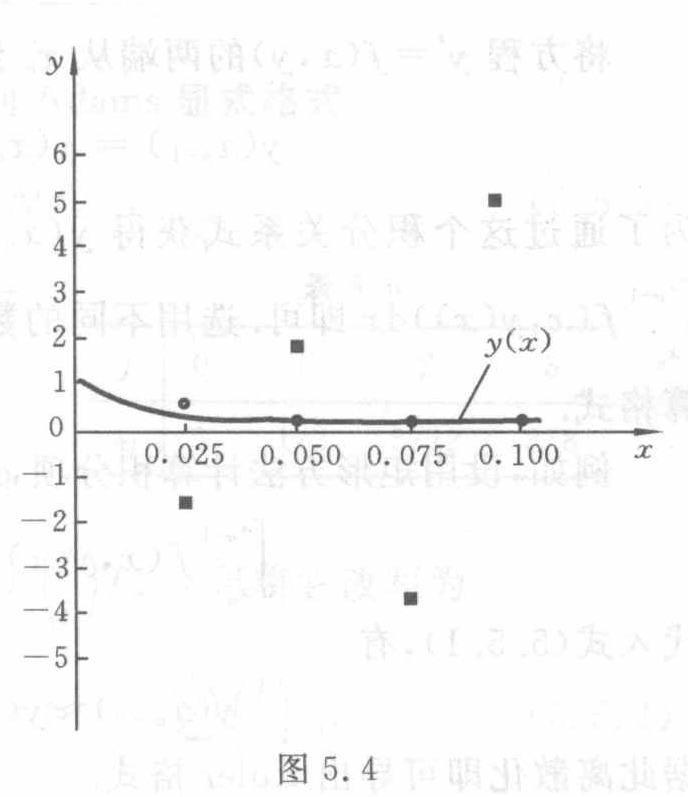
\includegraphics[width=0.85\linewidth,height=\textheight,keepaspectratio,alt={图 5.4 原图}]{verified/assets/ch05a/fig-5.4.png}

图 5.4（原图）：坐标系中画出衰减曲线 \(y(x)\)、正负交替且幅度增大的方形离散点，以及靠近横轴的圆形离散点。原图全部文字与刻度标签：\(x,y,y(x)\)；横轴 \(0.025,0.050,0.075,0.100\)；纵轴 \(-5,\allowbreak -4,\allowbreak -3,\allowbreak -2,\allowbreak -1,\allowbreak 0,\allowbreak 1,\allowbreak 2,\allowbreak 3,\allowbreak 4,\allowbreak 5,\allowbreak 6\)。点的说明随例 5.5 跨页续述。

\begin{quote}
\textbf{校注（agent 补充，原书文字/符号错误）}：例 5.5 原印``步长 \(h\) 应使 \(\tau\) 不超过 \(2\tau=0.02\)''，已经放大确认并保留。式 (5.4.13) 约束的是步长 \(h\)，应为``步长 \(h\) 应不超过 \(2\tau=0.02\)''；原句中的``使 \(\tau\)''使被约束量错置。
\end{quote}

